\documentclass[fleqn]{article}
\usepackage{amsmath, amssymb, amsthm}
\usepackage{commath}
\usepackage{siunitx}
\usepackage{tikz, pgfplots}
\usetikzlibrary{calc, hobby}
\usepackage{graphicx}
\usepackage{datetime}
\usepackage{ulem}
\usepackage{xcolor}
\usepackage{enumerate}
\setcounter{secnumdepth}{4}

\newcommand\numberthis{\addtocounter{equation}{1}\tag{\theequation}}

\newcommand{\AxisRotator}[1][rotate=0]{%
	\tikz [x=0.25cm,y=0.60cm,line width=.2ex,-stealth,#1] \draw (0,0) arc (-150:150:1 and 1);%
}

\theoremstyle{definition}
\newtheorem{example}{Example}
\newtheorem{definition}{Definition}

\theoremstyle{theorem}
\newtheorem{theorem}{Theorem}

\newenvironment{solution}
{\begin{proof}[Solution]\let\qed\relax}
	{\end{proof}}

%opening
\title{Lecture 7}
\author{Aakash Jog}
\date{\formatdate{18}{11}{2014}}

\begin{document}

\maketitle
%\setlength{\mathindent}{0pt}

\tableofcontents

\newpage
\section{Energy}

\subsection{Leibenitz's `Vis Viva'}

Based on experimental analyses, Leibenitz defined `vis viva' as the product of the weight of a body and its height above the ground. This definition contradicted Descartes, who defined the life force as the product of the mass of a body and the magnitude of its velocity. 

\subsection{Coriolis' Definition of Work}

Coriolis defined work as the multiplication of the displacement of a body, and the component of the force responsible for the displacement, in the direction of the displacement, or vice versa.

\begin{align*}
	\dif W &\doteq \overrightarrow{F} \cdot \dif \overrightarrow{r} \\
	\therefore W &\doteq \int_{\overrightarrow{r_A}}^{\overrightarrow{r_B}} \overrightarrow{F} \cdot \dif \overrightarrow{r}
\end{align*}

For a general body,
\begin{align*}
	W &=\int_{\overrightarrow{r_A}}^{\overrightarrow{r_B}} \overrightarrow{F_{\text{total}}} \cdot \dif \overrightarrow{r} \\
	&= \int_{\overrightarrow{r_A}}^{\overrightarrow{r_B}} m \dod{\overrightarrow{v}}{t} \cdot \dif \overrightarrow{r} \\
	\intertext{In Leibenitz's notation, $\dif t$ is a scalar. Therefore, we can move it around.}
	\therefore W &= \int_{\overrightarrow{r_A}}^{\overrightarrow{r_B}} m \dif \overrightarrow{v} \cdot \dod{\overrightarrow{r}}{t} \\
	&= \int_{\overrightarrow{v_A}}^{\overrightarrow{v_B}} m \dif \overrightarrow{v} \cdot \overrightarrow{v} \\
	\dif (v^2) &= 2 \overrightarrow{v} \dif \overrightarrow{v} \\
	\therefore W &= \int_{\overrightarrow{v_A}}^{\overrightarrow{v_B}} \dfrac{1}{2} m \dif (v^2) \\
	&= \dfrac{1}{2} m (v_B^2 - v_A^2) \\
	&= \dfrac{1}{2} m v_B^2 - \dfrac{1}{2} m v_A^2 \\
	&\doteq E_K(B) - E_K(A)
\end{align*}

\subsection{Gravitational Potential Energy}

\begin{align*}
	\overrightarrow{F_\text{total}} &= \overrightarrow{F_\text{gravitation}} + \overrightarrow{F_{\text{other}}} \\
	\overrightarrow{F_\text{total}} &= m \overrightarrow{g} + \overrightarrow{F_{\text{other}}} 
\end{align*}

\begin{tikzpicture}
	\draw [->] (0,0,0) -- (1,0,0) node [right] {$y$};
	\draw [->] (0,0,0) -- (0,1,0) node [above] {$z$};
	\draw [->] (0,0,0) -- (0,0,1) node [below] {$x$};
	
	\fill (-2,-3) circle [radius = 2pt] coordinate (C);
	
	\draw [->] (-2,-3) -- ++(-90:2) node [below] {$mg$};
	
	\draw [red, ->] (-2,-3) -- ++(-30:1) node [below] {$\dif r$};
	
	\draw [red, ->] (-2,-3) -- ++(-90:{cos 30}) node [below left] {$\dif z$};
	
	\coordinate (A) at (-4,1);
	\coordinate (B) at (2,-5);
	
	\draw (A) to [out=-30, in=150] (C) to [out=-30, in= 130] (B);
	
	\node at (A) [left] {A};
	\node at (B) [right] {B};
\end{tikzpicture}

\begin{align*}
	W(m\overrightarrow{g}) &= \int_{\overrightarrow{r_A}}^{\overrightarrow{r_B}} m \overrightarrow{g} \cdot \dif \overrightarrow{r} \\
	&= \int_{\overrightarrow{z_B}}^{\overrightarrow{z_A}} m g (\dif z) \\
	&= m g (z_A - z_B) \\
	&= m g z_a - m g z_B
\end{align*}

\begin{align*}
	W = \int_{B}^{A} \overrightarrow{F_{\text{total}}} \cdot \dif \overrightarrow{r} &= E_K(B) - E_K(A) \\
	\therefore \int_{B}^{A} \overrightarrow{F_{\text{other}}} \cdot \dif \overrightarrow{r} + W(m \overrightarrow{g}) &= E_K(B) - E_K(A) \\
	\therefore \int_{B}^{A} \overrightarrow{F_\text{other}} \cdot \dif \overrightarrow{r} &= (E_K(B) + m g z_B) - (E_K(A) + m g z_A) \\
	&= E_M(B) - E_M(A)
\end{align*}

\subsection{Spring Potential Energy}

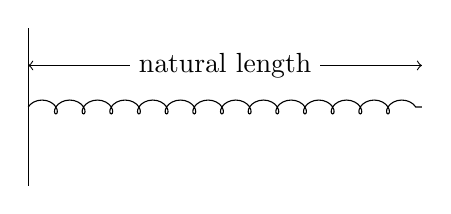
\begin{tikzpicture}
	\draw (0,1) -- (0,-1);
	
	\draw [decorate, decoration={coil, aspect=1}] (0,0) -- (0:5);
	
	\draw [<->, yshift=15] (0,0) -- (0:5) node [midway, fill=white] {natural length};
\end{tikzpicture}\\
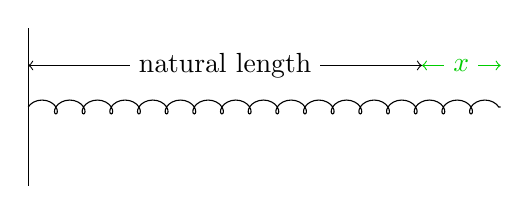
\begin{tikzpicture}
	\draw (0,1) -- (0,-1);

	\draw [decorate, decoration={coil, aspect=1}] (0,0) -- (0:6);

	\draw[green!80!black, <->, yshift=15] (0:5) -- (0:6) node [midway, fill=white] {$x$};

	\draw [<->, yshift=15] (0,0) -- (0:5) node [midway, fill=white] {natural length};
\end{tikzpicture}
\begin{equation*}
	F = k x
\end{equation*}
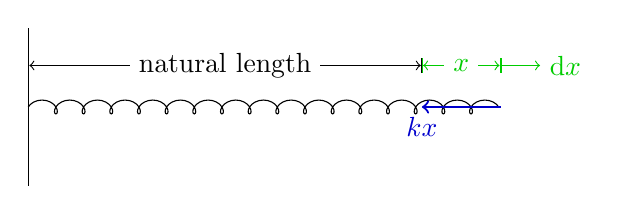
\begin{tikzpicture}
	\draw (0,1) -- (0,-1);

	\draw [decorate, decoration={coil, aspect=1}] (0,0) -- (0:6);

	\draw [|<->|, yshift=15] (0,0) -- (0:5) node [midway, fill=white] {natural length};

	\draw[green!80!black, |<->|, yshift=15] (0:5) -- ++(0:1) node [midway, fill=white] {$x$};
	\draw[green!80!black, |->, yshift=15] (0:6) -- ++(0:0.5) node [right] {$\dif x$};

	\draw[blue!80!black, ->, thick] (0:6) -- ++(180:1) node [below] {$kx$};

\end{tikzpicture}\\
The work done by the spring force is
\begin{align*}
	W(k) &= \int_{x_A}^{x_B} - k x \dif x \\
	&= \dfrac{1}{2} k x_A^2 - \dfrac{1}{2} k x_B^2
\end{align*}

\begin{align*}
	W = \int_{B}^{A} \overrightarrow{F_{\text{total}}} \cdot \dif \overrightarrow{r} &= E_K(B) - E_K(A) \\
	\therefore \int_{B}^{A} \overrightarrow{F_{\text{other}}} \cdot \dif \overrightarrow{r} + W(m \overrightarrow{g}) +W(k \overrightarrow{x}) &= E_K(B) - E_K(A) 
\end{align*}
\begin{align*}
	\therefore \int_{B}^{A} \overrightarrow{F_\text{other}} \cdot \dif \overrightarrow{r} &= (E_K(B) + m g z_B + \dfrac{1}{2} k x_B^2)
	- (E_K(A) + m g z_A + \dfrac{1}{2} k x_A^2) \\
	&= E_M(B) - E_M(A)
\end{align*}



\subsection{Examples}

\begin{example}
	Find $h_{\text{min}}$ so that the mass can complete the circular motion.
	\begin{tikzpicture}
		\draw (-8, 10) to [out=-90, in=180] (0, 0);
		\draw (0, 4) circle [radius=4];
		\draw [dashed] (0,4) -- ++(35:4) node [midway, fill=white] {$R$};
		
	%	\coordinate (0,8) 
	
		\draw [decorate, decoration={brace, mirror}, xshift=-10] (-8,10) -- (-8,0) node [midway, left] {$h$};
		
		\draw (0,7.75) circle [radius=0.25];
		
		\draw [->] (0,7.75) -- ++(-90:1) node [below] {$mg$};
		
		\draw [->] (0,7.75) -- ++(90:1) node [above] {$N$};
		
		\draw [dashed] plot (\x, 8) node [right] {$z = 0$};
	\end{tikzpicture}
\end{example}
\begin{solution}
	\begin{align*}
		m g + N = m \dfrac{v^2}{R}
		\intertext{At $h_{\text{min}}, N = 0$}
		\therefore v = \sqrt{g R}
	\end{align*}
	$E_M = $ constant \\
	Therefore, comparing mechanical energy at A and B,
	\begin{align*}
		m g (h - 2R) &= \dfrac{1}{2} m v^2 \\
		\therefore h_{\text{min}} = \dfrac{5}{2} R
	\end{align*}
\end{solution}

\begin{example}
	Find the average force exerted by the sand on the body.
	%\includegraphics[width=4in]{IMG_4132.JPG} 
	
	\resizebox{\textwidth}{!}
	{
	\begin{tikzpicture}
		\draw [rounded corners=10] (0,0) coordinate(O)
		\foreach \i in {1,...,10} 
		{
			to ++(-1, rnd)
		} coordinate (A);
	
		\node [below left] at (A) {A};
	
		\draw (A) -- ++(180:2) -- ++(90:0.5) coordinate (A');
		
		\draw (A') -- ++(-90:0.25) coordinate (spring beginning);
		\draw [decorate, decoration={coil, aspect=1}] (spring beginning) -- ++(0:1.75) coordinate (spring end);
		
		\fill (spring end)+(0.25,0) circle [radius=0.25];
		
		\draw [rounded corners] (O) to [out=0, in= 180] ++(4, -2) -- ++(0:1) coordinate (B) -- ++(-90:3) -- ++(0:3) coordinate (B');
		
		\node [below left] at (B) {B};
		
		\draw [dashed] (B') -- ++(0:1) coordinate (C) -- ++(0:2) node [midway, below] {sand};
		
		\node at (C) [above right] {C};
		
		\draw [dotted] (B)+(0,0.25) to [out = 0, in = 110] (C) to ++(-70:0.5) coordinate (C');
		
		\fill (B) circle [xshift=0.25cm-10pt, yshift=0.25cm, radius = 0.25];
		
		\fill (C') circle [radius = 0.25];
		
	\end{tikzpicture}
	}
	
	\begin{align*}
		m &= \SI{2}{\kilogram} \\
		h_1 &= \SI{3}{\metre} \\
		h_2 &= \SI{3}{\metre} \\
		l &= \SI{10}{\metre} \\
		k &= \SI{1000}{\newton\per\metre} \\
		x &= \SI{40}{\centi\metre} \\
		\mu_k &= 0.2
	\end{align*}
\end{example}
Consider the datum of gravitational potential energy at A.
\begin{align*}
	W(\overrightarrow{F_{\text{other}}}) &= E_M(B) - E_M(A) \\
	\therefore 0 - \mu_k m g l &= (\dfrac{1}{2} m v_B^2 + m g (-h1) + 0) - (0 + 0 + \dfrac{1}{2} k x^2)\\
	\therefore v_B = 10 \text{ m/s}
\end{align*}
At point C,
\begin{align*}
	E_M &= \dfrac{1}{2} k x^2 + m g (h_1 + h_2) - \mu_k m g l\\
	&= \dfrac{1}{2}(1000)(0.4)^2 + (2)(10)(6) - (0.2)(2)(10)(10)\\
	&= 160 \text{ J}
\end{align*}
This energy is is dissipated by the action of the force of the sand.
\begin{align*}
	(F_{\text{sand}})(0.1) &= 160 \\
	\therefore F_{\text{sand}} &= 1600 \text{ N}
\end{align*}

\begin{example}
	{\color{blue}$\overrightarrow{F'}$} is always at 30 degrees from horizontal.\\
	{\color{red}$\overrightarrow{F}$} is always tangential to the hemisphere.\\
	\begin{tikzpicture}
		\draw (-5,0) arc [radius = 5,start angle =-180, end angle=0];
		\draw [dashed] (-5,0) -- (5,0);
		\draw [dashed] (0,0) -- (0,-5);
		
		\draw [dashed] (0,0) -- ++(220:5);
		\node at ({220 + (270-220)/2}:1) {$\theta$};
		
		\fill (220:5) circle [radius=2pt];
		
		\draw [green!80!black, ->] (220:5) -- ++(-50:0.5) node [below left] {$\dif \overrightarrow{r}$};
		
		\draw [red, ->] (220:5) -- ++(-50:1) node [below] {$F$};
		
		\draw [blue, ->] (220:5) -- ++(30:1) node [right] {$F'$};
	\end{tikzpicture}\\
	Find the work done by both forces.
\end{example}

\begin{solution}
	{
	\color{red}
	\begin{align*}
		W(F) &= \int_{A}^{B} \overrightarrow{F} \cdot \dif \overrightarrow{r} \\
		&= \int_{A}^{B} F \dif r \\
		&= F \int_{A}^{B} \dif r \\
		&= F(\pi r)
	\end{align*}
	}
	{
	\color{blue}
	\begin{align*}
		W(F') &= \int_{A}^{B} \overrightarrow{F} \dif \overrightarrow{r} \\
		&= \int_{A}^{B} F' \dif r \cos \left(\theta + \dfrac{\pi}{6}\right) \\
		&= F' \int_{A}^{B} \cos \left(\theta + \dfrac{\pi}{6}\right) \dif r \\
		&= F' \int_{\dfrac{\pi}{2}}^{- \dfrac{\pi}{2}} \cos \left(\theta + \dfrac{\pi}{6}\right) (-R \dif \theta) \\
		&= F' R \int_{-\dfrac{\pi}{2}}^{\dfrac{\pi}{2}} \cos \left(\theta + \dfrac{\pi}{6}\right) \dif \theta \\
		&= F' R \sin \left(\dfrac{2 \pi}{3}\right) - F' R \sin \left(\dfrac{-\pi}{3}\right) \\
		&= F' R \sqrt{3}
	\end{align*}
	}\\
	The work done by {\color{blue} F'} is the same, even if the body is taken directly from A to B.
\end{solution}
\subsection{Work Done by Friction}

\begin{align*}
	W(\overrightarrow{F_{\text{total}}}) &= \dfrac{1}{2} m v_f^2 - \dfrac{1}{2} m v_i^2 \\
	\int_{x_A}^{x^B} - f \dif x &= \int_{0}^{x} \mu_k m g \dif x \\
	\therefore - \mu_k m g x &= \dfrac{1}{2} m v_f^2 - \dfrac{1}{2} m v_i^2
\end{align*}

\subsection{Friction on an Inclined Plane}

%\begin{tikzpicture}
%	
%\end{tikzpicture}

\begin{align*}
	\int \overrightarrow{F_{\text{other}}} \cdot \dif \overrightarrow{r} &= E_M(f) - E_M(i) \\
	\therefore W(\overrightarrow{N}) + W(\overrightarrow{f}) &= \dfrac{1}{2} m v_f^2 -m g l \sin \theta \\
	\therefore - \mu_k m g \cos \theta l &= \dfrac{1}{2} m v_f^2 - m g l \sin \theta \\
	\therefore - \mu_k m g x &= \dfrac{1}{2} m v_f^2 - m g l \sin \theta
\end{align*}

\end{document}